\chapter{Document Retrieval}
\label{chap:docret}

The term document retrieval refers to the task of finding relevant information to user queries in a large set of records (documents). 
% Therefore, the document retrieval system operates over a database of records, which for this thesis are described in \ref{chap:data}.
One can think of document retrieval as a search in a vast database of documents. 
In this view, web search services, such as Google, are also a form of document retrieval. 
In this case, the database of documents is all the accessible web pages on the internet.

For our uses, the query is the claim to be fact-checked, and the document database is a collection of relevant documents, which we call knowledge base. 

In this chapter, we define the task of document retrieval and introduce traditional and novel (neural) approaches to solving it.
After describing the traditional word-weighting approaches, we examine crucial concepts behind the used neural models.
We then describe the framework which allows us to use the neural models on the document retrieval task.
We then propose a way of applying the models to the document retrieval task.
TODO -- remove one of the two previous sentences.

\section{Formal Description}
\label{sec:formal_descr_dr}
The task can be formally described \citep{two-tower} using a scoring function (sometimes referred to as ranking function) %article before ranking maybe
\begin{equation}
        f_\mathcal{D}\colon\mathcal{D}\times\mathcal{Q}\rightarrow\R
        \label{eq:formal_descr_dr}
\end{equation}
that maps a document-query pair $(d, q)$ to a score $f(d,q)$. 
Then, typically, the documents in pairs with the highest scores are considered to be the proposed solution to the task. 

As mentioned above, this definition also fits descriptions of a range of other tasks such as open-domain question answering \citep{wiki-retrieval} or recommendation systems.

\section{Approaches to Document Retrieval}

The organizators of \textbf{T}ext \textbf{Re}trieval \textbf{C}onference (TREC) \citep{trec-2020} classify retrieval methods into three categories (with examples):
\begin{itemize}
        \item Traditional -- TFIDF, BM25
        \item Neural Networks using Language Modeling (NNLM) -- BERT-based
        \item Neural Networks -- others
\end{itemize}
We explore NNLM and traditional approaches, emphasizing the NNLM approach while using the latter as the baseline.
``Neural Networks'' is reserved for methods that use neural networks only in some parts of its implementation (such as word embeddings) and do not rely explicitly on language modeling.
We do not explore such methods in this thesis, and therefore, by neural approach, we refer to NNLM methods
While both work on entirely different principles, we will use both to generate an indexed version of the knowledge scope.

This chapter further introduces the most common document retrieval methods and new models with great potential while explaining the main points of the theoretical background.

\section{Traditional Approaches}

Traditional approaches covered are weighting schemes, assigning a query-dependent score to each word in each document in the database.

\subsection{TFIDF}

The traditional approaches are motivated by the intuition that relevant documents will contain the same words as those present in the query. 
Longer documents are at an advantage since there is a higher chance of the relevant words being present, so the term count is often normalized by the number of all terms in the document.
This simple metric is called term frequency (TF). 

TF can be ineffective if some of the terms in the query are very common in the document database.
This issue is resolved by introducing inverse document frequency, which informs how common the term is across all the documents.
The base version of IDF:
\begin{equation}
        \text{idf}(t, D)=\log{\frac{\abs{D}}{\abs{\{d\in D: t\in d\}}}}\ .
\end{equation}

% If we combine these two metrics
Multiplying these two metrics, we get the TFIDF weight of term $t$ in document $d$ in document database $D$:
\begin{equation}
        \text{tfidf}(t,d,D)=\text{tf}(t,d)\cdot\text{idf}(t,D)\ .
\end{equation}

\begin{figure}[!htb]
	\centering
	\begin{minipage}{.5\textwidth}
		\centering
		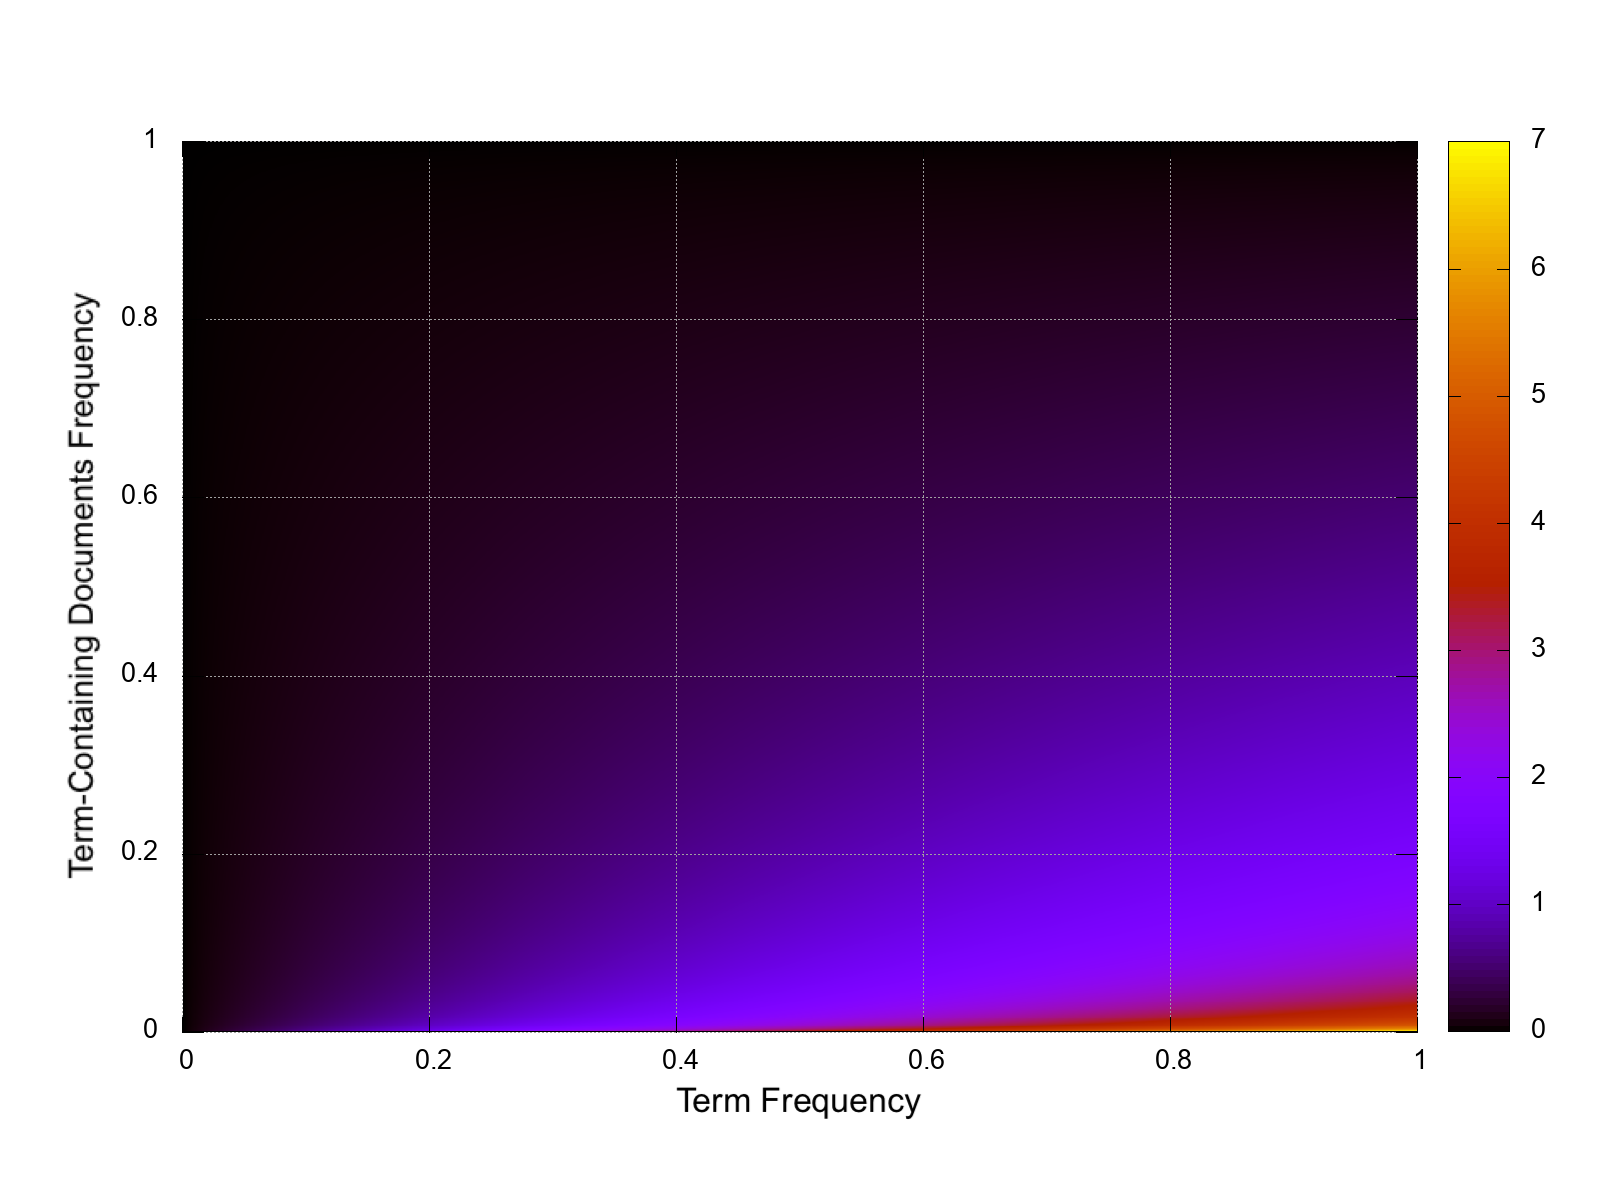
\includegraphics[width=\linewidth]{tfidf_map.png}
	\end{minipage}%
	\begin{minipage}{.5\textwidth}
		\centering
		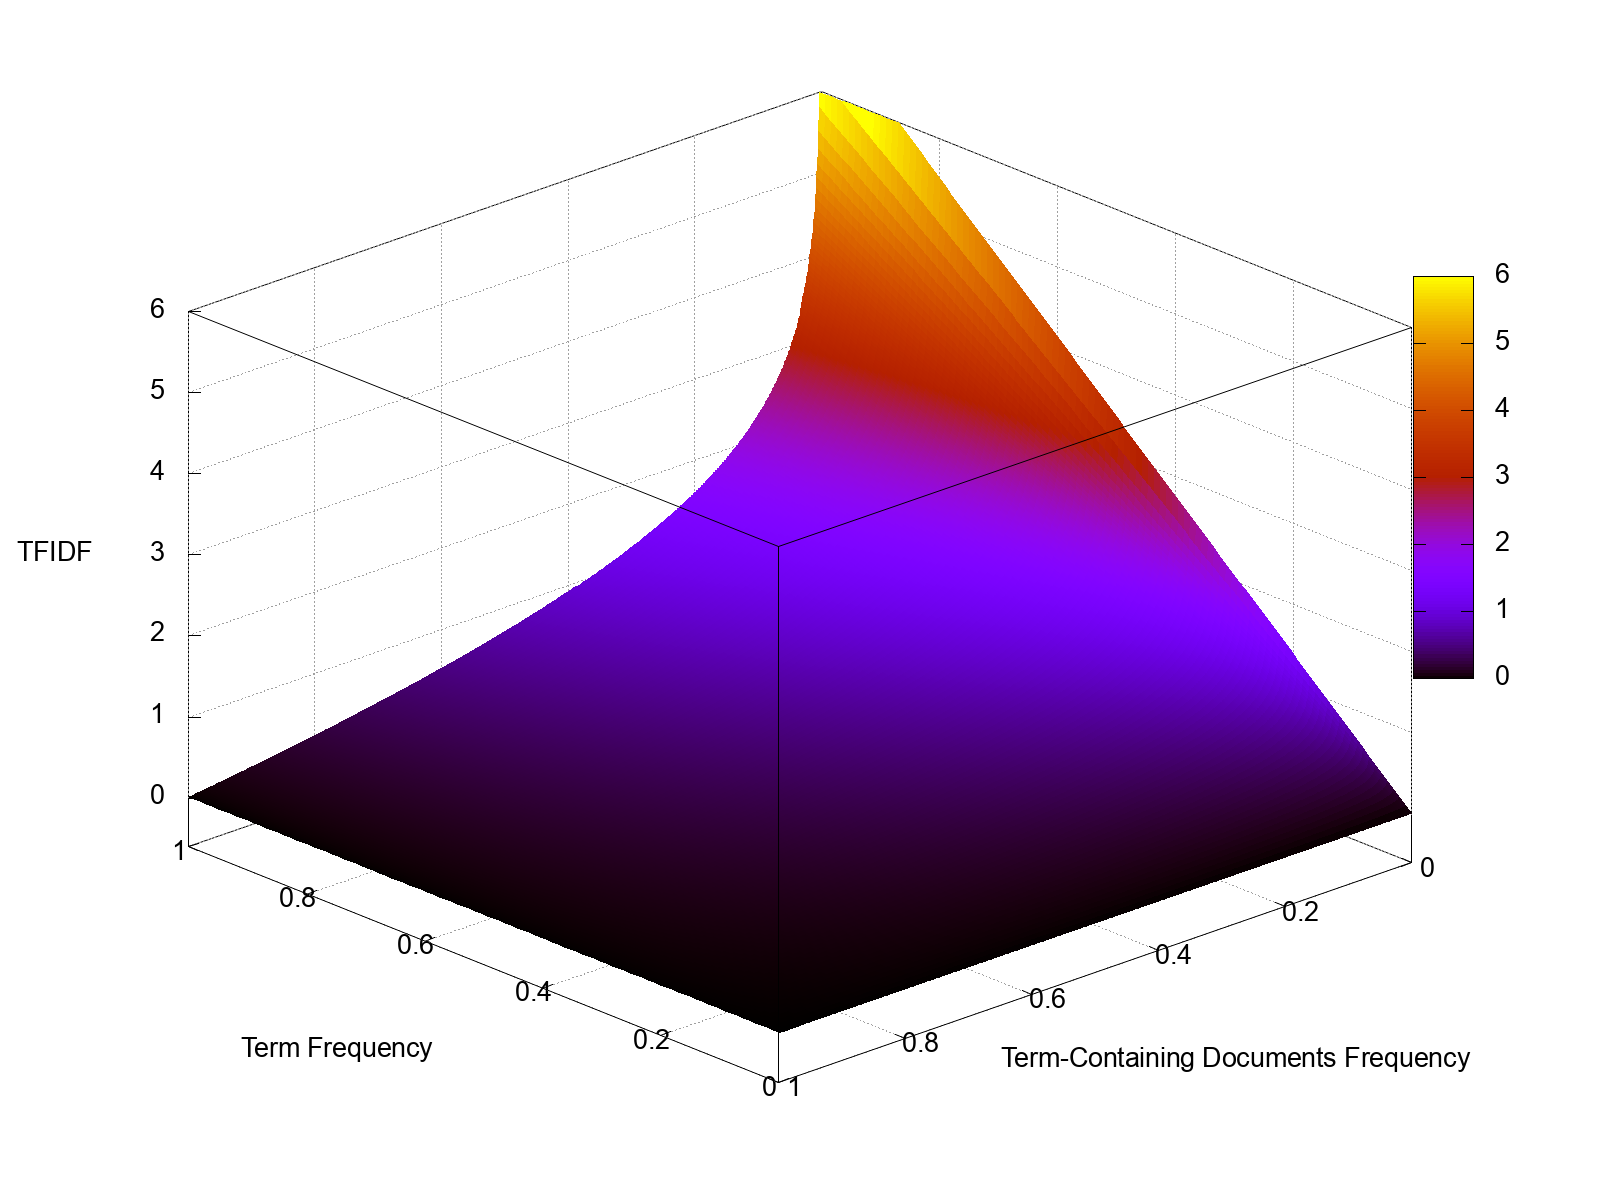
\includegraphics[width=\linewidth]{tfidf.png}
	\end{minipage}
        \caption[Visualization of TFIDF]{Visualization of TFIDF depending on the term frequency and the frequency of the documents containing the term.}
\end{figure}

We have explained how to compute a term's weight (``importance'') for a specific document.
The intuitive formula for query score $f(q, d)$ is then
\begin{equation}
        f_D(q, d)\approx\sum_{t \in q}\text{tfidf}(t, d, D)\ .
\end{equation}
TFIDF is called a weighting scheme precisely for this reason.

Since % term frequency and therefore tfidf is zero when 
$$t\notin d \hspace{1mm}\Rightarrow\hspace{1mm} \text{tf}(t, d) = 0 \hspace{1mm}\Rightarrow\hspace{1mm} \text{tfidf}(t, d, D) = 0\ ,$$
we know that only words in the corpus' vocabulary are important, and thus we can precompute the TFIDF values for each document, and word from the corpus' vocabulary.
We obtain $|D|\times {vocabulary\_size}$ matrix $V$ of TFIDF values.
%This formula can be improved -- in this form, it favors longer queries $q$. % DOES IT? TODO
%We can also precompute the TFIDF values for each document and vocabulary word in the corpus.
%Thus we obtain $|D|\times {vocabulary\_size}$ matrix $V$ of TFIDF values.
Here, to simplify length normalization, we normalize the matrix V so that each row has a unit norm.
This step removes the need for normalization in the TFIDF formula, and we may use raw term count instead of the normalized frequency.
To get the relevance of each document to the query $q$, that is $f_D(q, d)$, we first represent the query $q$ as a bag of words vector (BOW), corresponding to the columns of our precomputed TFIDF matrix $V$, ignoring words that appear only in the query.
The resulting score is then the normalized (not to favor long queries) dot product of a row of the matrix and the BOW representation of the query $q$ denoted $\vec{q}$.
We can obtain the scores for every query document pair by matrix multiplication:
\begin{equation}
        f_D(q, d) = \frac{V\vec{q}}{|\vec{q}|} \in \R^{|D|}\ ,
\end{equation}
provided that matrix $V$ is row-normalized (euclidian norm of each row is equal to one).
Please note that this is equivalent to computing the cosine similarity for each document and query vector pair.

This function is one of the first and still widely used \citep{Beel2016} weighting schemes for document retrieval. 

Over the years, multiple versions of the TFIDF approach appeared, differing slightly in formulas or weights of the factors. One of such versions is Best Match 25. %questionable TODO
% maybe put the last sentence as the last sentence of the whole section

\subsection{Best Match 25 (BM25)}

%The following is 
A more complex term weighting scheme is Best Match 25 \citep{bm25}:
%One of the best performing versions \citep{bm_vs_tfidf} is Best Match 25 (BM25) by \cite{bm25}.
%The original formula is:
\begin{equation}
\text{BM25}(q, d) = 
        \sum_{t\in q}
        \text{idf}(t, d)
        \cdot \frac{(k_1 + 1)\cdot\text{c}(t, d)}{k_1(1-b + b \cdot (L_d / L_{avg})) + \text{c}(t, d)} 
        \cdot \frac{(k_3 + 1)\cdot\text{c}(t, q)}{k_3 + \text{c}(t, q)}
\ ,
\end{equation}
where $\text{c}(t,d)$ is the raw count of the term $t$ in the document $d$. $L_d$ and $L_{avg}$ are the current document's length the average document length, respectively.

The first term is IDF.
The second term is TF with two tuning parameters $k_1$ and $b$. Parameter $k_1$ corresponds directly to TF scaling, while parameter $b$ corresponds to scaling by the inverse of the document's length.
The third term follows the same idea as the second term, but the $b$ parameter equivalent is unnecessary since we only have one fixed query.
It shows \citep{schutze2008introduction} that this term is only valid for longer queries $q$, such as whole paragraphs. 
\begin{figure}[h!]
    \centering
    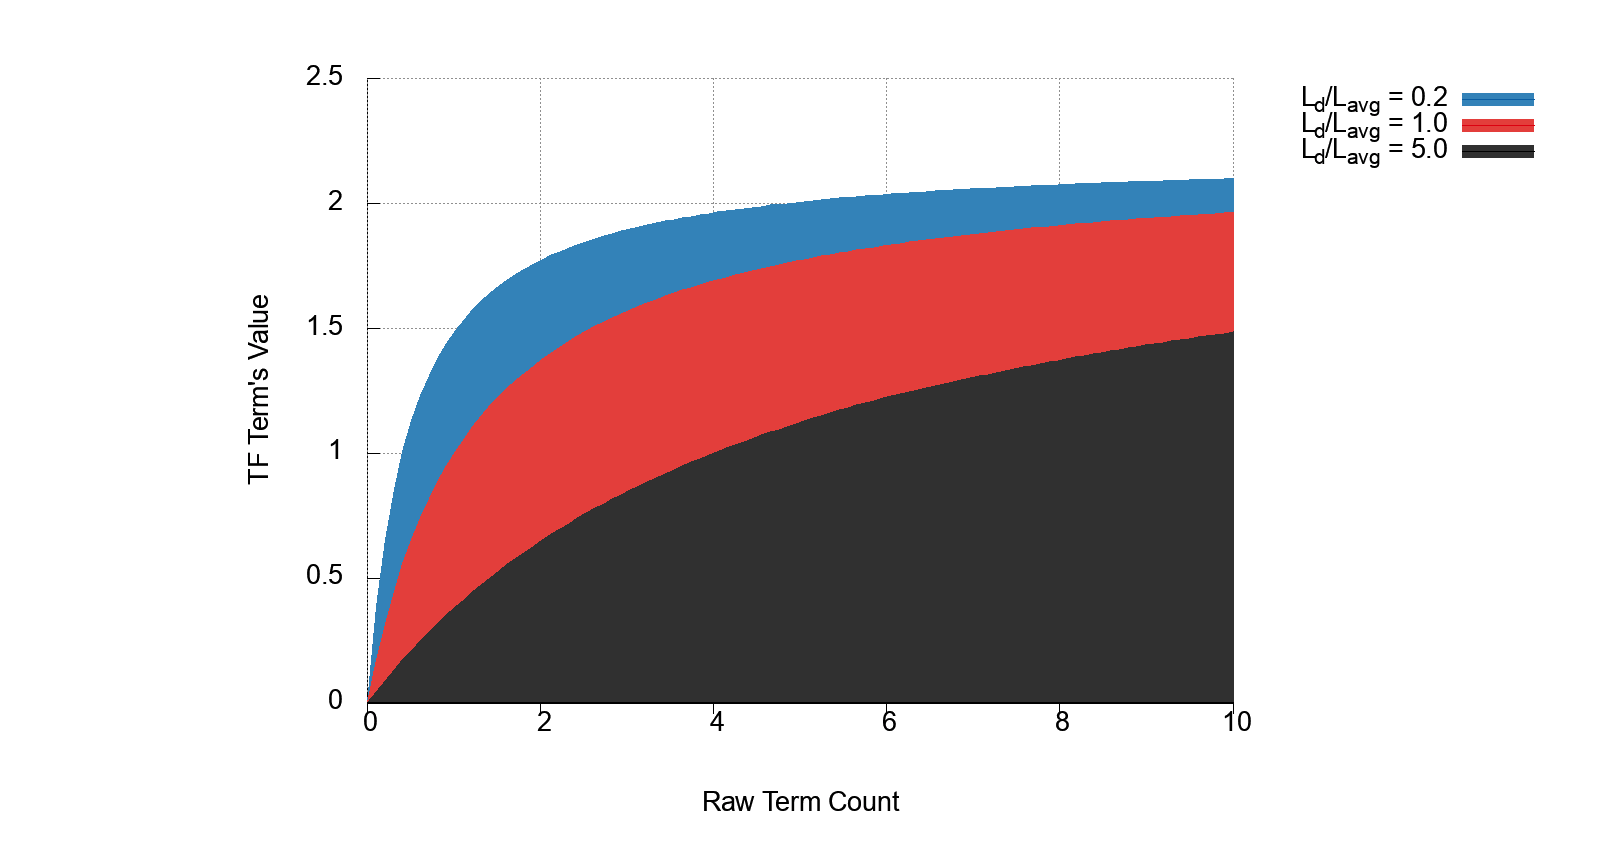
\includegraphics[width=.9\textwidth]{bm25.png}
    \caption[BM25 TF Visualization]{TF term's relation to the length of the current document for $k=1.2$ and $b=0.75$.}
\end{figure}

Since this weighting scheme introduces tunable parameters, it can be trained on data. If the data is not available, \citet[Section 11.4.3]{schutze2008introduction} recommend using $k_1, k_3 \in [1.2;2]$ and $b=0.75$.

%TODO problem with long documents - BM25+ http://sifaka.cs.uiuc.edu/~ylv2/pub/cikm11-lowerbound.pdf

\subsubsection{Final Thoughts}

Some of the apparent disadvantages of traditional approaches are the lack of semantic meaning that comes from the independence on the word order and the exact word matching. % independence???
The former may be improved by using n-grams and the latter using character-level features instead of words, especially in inflected languages such as Czech.
On the other hand, TFIDF is, to this day, a very well-performing low-computation cost ranking function, and as reported by \cite{weak-baselines}, BM25 (if tuned well) is still a solid baseline capable of beating even much more complex neural models.

\section{Neural Approaches}
\label{sec:neural_approaches}

Neural approaches using language modeling are models trained on predicting the correct word given some text before.  % maximizing the likelihood of correct word prediction in a text. 
% More precisely, it is a conditional language modeling since the prediction also depends on provided input.
Recurrent neural network (RNN) architecture was traditionally used for this task.
The RNN was fed encoded tokenized input, returning a hidden state which was next fed into the RNN again along with the next input token.
% The RNN was fed encoded tokenized input, and the RNN predicted the next token as depicted in Figure \ref{fig:lec6_slide23}.
Its hidden states could also be used to encode the input into a fixed-length vector representation, which can be further used to either classify the input or use another RNN (decoder) to generate another sequence.
Intuitively, the vector contains the meaning of the original input. 
Such an approach is the Sequence to Sequence (seq2seq or encoder-decoder) model architecture \citep{seq2seq} with significant use-case in machine translation.

As an improvement to the seq2seq models, the attention mechanism was introduced by \citet{first-attention}.
The authors viewed the RNNs as a bottleneck to improving the model's performance.
They proposed an automatic method of enriching parts of the input with other relevant parts of the input, eliminating the need to process the input as a whole.
The attention mechanism is in-depth described in subsection \ref{subsec:attention}.

% TODO check if this sits nicely
\begin{figure}[b!]
        \centering
        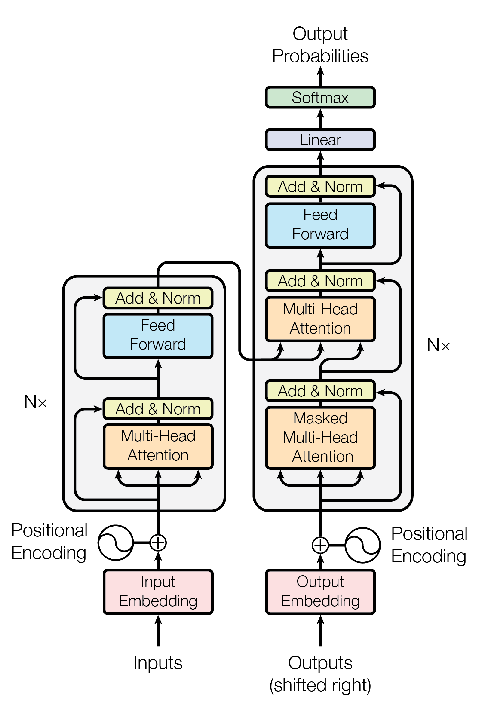
\includegraphics[width=.5\textwidth]{transformer.pdf}
        \caption[Transformer Model Architecture]{The transformer model architecture. Reprinted from \citep{attention-is-all-you-need}.}
        \label{fig:transformer}
\end{figure}

The research paper ``Attention Is All You Need'' by \citet{attention-is-all-you-need} improved the RNN-based seq2seq by introducing the transformer architecture, depicted in Figure \ref{fig:transformer}, by substituting the RNN by multiple ``encoder blocks'', that is, attention layer and feedforward network with skip-connection. 
This resulted in simpler architecture (RNN architectures tend to become very complex when trying to avoid the vanishing gradient problem), parallelization of the computation, and, most importantly, an improved performance. 
The improvement showed that the attention mechanism was crucial to the past achievements of the seq2seq models, hence the paper's name.
%On the other hand, the attention mechanism also introduces quadratic time complexity, which acts as a bottleneck in applications, where a longer input is required.
%That is why the transformer models are generally used with fixed 512 token input length.
%That might be adequate for most applications, but in document retrieval, the documents might get truncated.
%Also, the omission of RNNs meant that the input is not longer sequentially processed. 
%While allowing for parallelization, the position information is lost, and therefore position embedding is added. 
% NAKONIEC SOM TO POUZIL INDE ALE NECHAL AJ TU NECH TO VIEM POROVNAT
% neviem kam to quadratic TODO TODODODODODODOD TOTO ASI CELA DRUHA POLKA FAKT PREC TO SA TAM NEHODI

Then \textbf{B}idirectional \textbf{E}ncoder \textbf{R}epresentations from \textbf{T}ransformers (BERT) \citep{bert} model was introduced. It was ``designed to pre-train deep bidirectional representations from unlabeled text by jointly conditioning on both left and right context in all layers''. 
The model can then be fine-tuned on a specific task using a small amount of labeled data and one additional output layer. 

This was a brief description of how a sequence of research papers -- ``Sequence to Sequence Learning with Neural Networks'' \citep{seq2seq}, ``Neural Machine Translation by Jointly Learning to Align and Translate'' \citep{first-attention}, ``Attention Is All You Need'' \citep{attention-is-all-you-need}, and ``BERT: Pre-training of Deep Bidirectional Transformers for Language Understanding'' \citep{bert} -- led to a shift from RNN-based NLP approaches to, now SOTA, BERT-based approaches.
This research focus is sometimes referred to as BERTology.

In the following sections, we will explain the concepts mentioned above in greater detail.

%The authors trained the model on a large unlabeled corpus using two tasks. 
%The first was to predict random masked words, and the second classified whether the second sentence of two selected sentences immediately follows the first one.
%It is a language modeling encoder capable of non-supervised learning 

\subsection{Word Vectors}

Unlike traditional approaches, neural networks require numbers as their inputs.
Therefore the words (tokens) have to be encoded into a numeric representation with a fixed length.
The word encoding is just another linear layer (with $vocab\_size \times embedding\_dim$ weight matrix), which can be trained from scratch, or one could use pre-trained (for example \citep{glove}) word vectors (the rows of the matrix).

\subsection{Attention Mechanism}
\label{subsec:attention}

The main feature of the transformer models is the attention mechanism. It adjusts each token's embedding based on all the other tokens present in the current input.
This is done by computing three different linear projections of the original input tokens and then, based on certain similarities, combining them back together. 
The attention mechanism is also referred to as self-attention since all the tokens in one input attend to the same input.

The projections are computed using trainable matrices $W_Q$, $W_K$, and $W_V$, producing queries $Q$, keys $K$, and values $V$. Then, we compute the dot product (``similarity'') between the keys and the queries $QK^T$, illustrated in Figure \ref{fig:self-attn}.
The result is normalized by the inverse factor of the square root of the projection dimension. 
Then softmax is applied, and the result is used as the weights for the weighted average of all value vectors. To put it into an equation: 
\begin{equation}
  \text{Attention}(Q,K,V) = \text{softmax}\left(\frac{QK^T}{\sqrt{d}}\right)V\ .
  \label{eq:attention}
\end{equation}
Therefore, for every token, the result is the weighted average of all the value vectors, based on the similarity between the queries and the keys. 
The result is called scaled dot-product attention.

The computation is performed multiple times in parallel with independent projection matrices to make the mechanism more robust.
The results are then concatenated and projected into the final dimensionality.
This extended attention is called multi-head attention.
The intuition is that different heads might learn to attend to different patterns and meaning subspaces.

% TODO check if correct position
\begin{figure}[!htb]
	\centering
	\begin{minipage}{.49\textwidth}
		\centering
		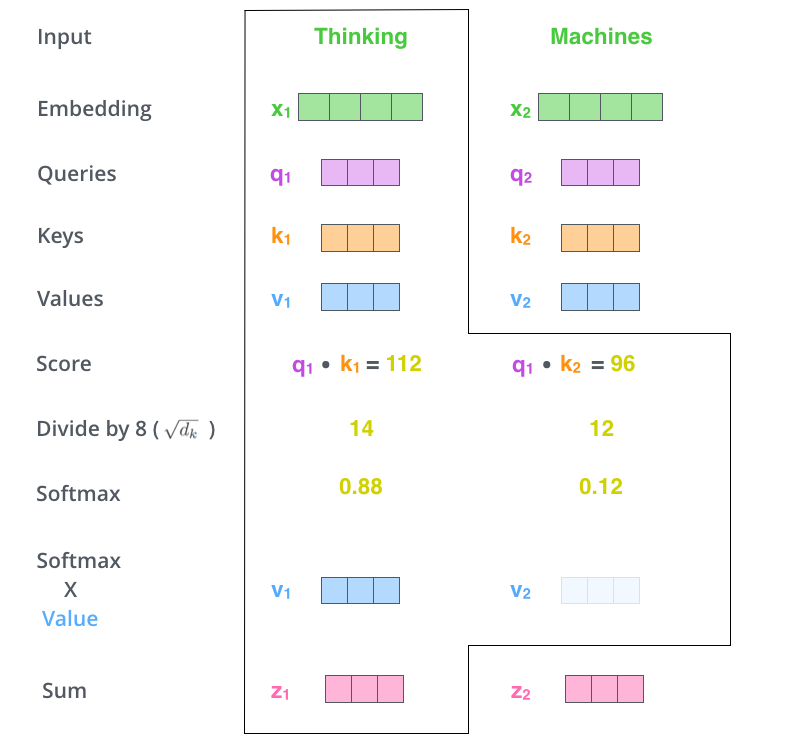
\includegraphics[width=\linewidth]{self_attention_output.png}
                \caption[Attention Mechanism Computation Example]{Example of self attention mechanism with projection dimension 64 and the input ``Thinking Machines''. Reprinted from \citep{illustrated-transformer}.}
	\end{minipage}
        \hfill
	\begin{minipage}{.49\textwidth}
		\centering
		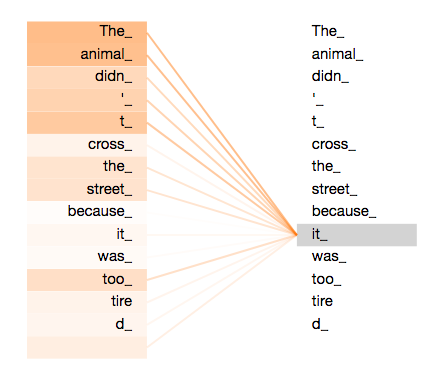
\includegraphics[width=\linewidth]{self_attention_visualization.png}
                \caption[Attention Values Visualization]{Self-attention mechanism example, where the token for word ``it'' is paying attention to ``the animal'', effectively being substituted for it. The orange color represnts the values from $QK^T$. Reprinted from \citep{illustrated-transformer}.}
                \label{fig:self-attn}
	\end{minipage}
\end{figure}

\subsection{Transformer and BERT}

As mentioned earlier, the transformer architecture no longer uses RNNs.
The omission meant that the input is not longer sequentially processed.
While allowing for better performance through parallelization, the position information is lost, and therefore the information has to be added to each input token.
The solution is embedding the position into the same dimension as the word (token) vectors and then adding the positional embedding to the token's embedding.
The position embedding is fixed, non-trainable, and defined as a vector of trigonometric functions applied to the position index, depicted in Figure \ref{fig:pos_emb}.
The authors provide a detailed explanation in \citep[Section 3.5]{attention-is-all-you-need}.

%TODO check position
\begin{figure}[!htb]
        \centering
        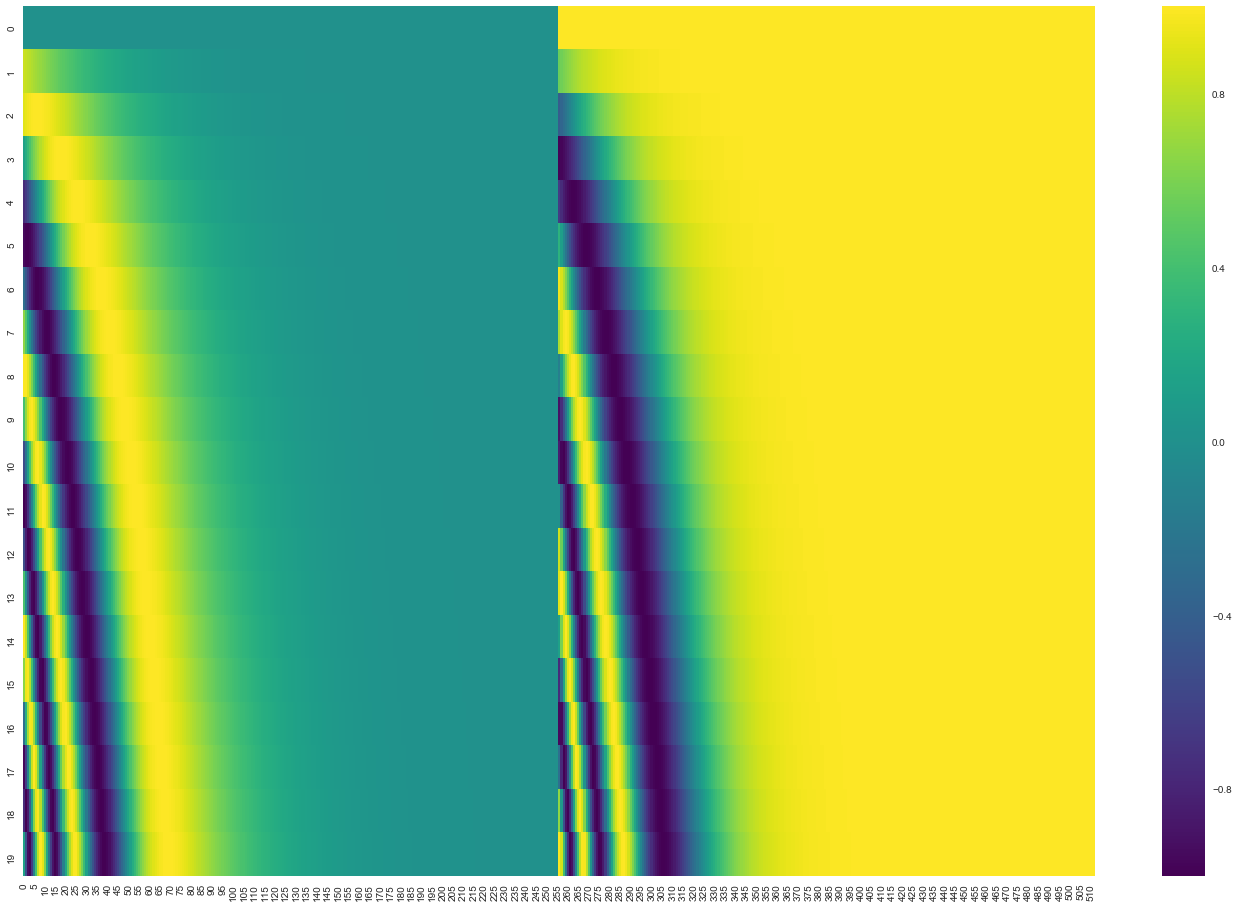
\includegraphics[width=\textwidth]{transformer_positional_encoding.png}
        \caption[Positional Encoding of Transformer's Input]{Transformer positional encoding as described in \citep{attention-is-all-you-need}. Input length is 20 tokens with the embedding dimension of 512. For better visualization, the originally alternating $\sin$ and $\cos$ functions are divided to the left and right half, respectively. Reprinted from \citep{illustrated-transformer}.}
        \label{fig:pos_emb}
\end{figure}

While seq2seq architecture can work with arbitrary sequence types, BERT is a language model working with text input. 
Specifically, it is just the encoder part of the seq2seq architecture, meant for computing real-valued fixed-length vector representation of the input that can further be used by other neural models (usually shallow fully-connected feedforward networks).
The encoder is trained on a large amount of unlabeled text data (corpus) in a phase called pre-training.
This phase, accounting for a great number of the model's parameters ($\approx$ 110 million in its base form), consumes a significant amount of power. 
The model can then be fine-tuned, that is, trained for the task we want to apply it on, such as Named Entity Recognition (NER) \citep{ner}, Natural Language Inference (NLI) \citep{nli-bowman,nli-williams}, or Question Answering (QA) \citep{squad}. 
This is done by usually adding one fully connected layer after the encoder output and relatively short training (of all parameters) with the usage of a smaller amount of labeled data. 

Intuitively, the pre-training ``teaches'' the language and word meanings while the fine-tuning only ``explains'' the final task to the model.

\subsection{Transformer's Computational Limits}

While the benefits of the attention mechanism are undeniable \citep{attention-is-all-you-need}, on the other hand, it introduces quadratic time and space complexity by employing the ``one on one'' approach coupled with the non-linear softmax operation, which prevents various optimization techniques to be applied.
That is why the attention mechanism acts as a bottleneck in applications, where a longer input is required.
Transformer models, therefore, generally have the input length fixed to 512 tokens (shorter inputs are padded, longer truncated).
That might be adequate for most applications, but in document retrieval, valuable information might get lost.

Other parts of the transformer architecture too use a large amount of memory. During training, the activations of every encoder layer have to be stored for back-propagation. Feedforward layers in the encoder blocks are also nontrivially large.

\subsection{BERTology}

The research focus on BERT-like models resulted in many papers introducing minor and major changes to the BERT's architecture.
We will focus on modifying the attention mechanism so that longer inputs are no longer the limiting factor during computation.
%We will focus on the ones modifying the attention mechanism in such a way that larger inputs are no longer the limiting factor during computation. 

\subsubsection{Longformer}

The Longformer architecture \citep{longformer} represents the simplest form of the attention mechanism modification.
Instead of computing the whole $QK^T$, only certain regions (usually specific diagonals) are calculated, thus reducing the model time complexity allowing for longer inputs.

The authors proposed attention windows that ensured that each token attended only to a fixed number of the neighboring tokens. 
Given multiple encoder blocks of the transformer architecture (Figure \ref{fig:transformer}), each token eventually attends to all the input tokens, similarly to CNNs.  
Additionally, a ``dilated'' window attention was used, where the window contains gaps of parametrized size. 
The authors claim that using different sizes of dilation per attention head proved to be beneficial.

In different applications the model performs better with different attention patterns and it might require that some positions attend to the whole input; for example, in question answering, it is essential to attend to the question.
Thus, the authors use another set of projections in the attention mechanism (initialized from the windowed attention) called global attention.
It arises by allowing some positions to attend to the whole input and making the whole input sequence attend to them, as in Figure \ref{fig:longformer_attention}.  %TODO check 

% TODO check position
\begin{figure}[!htb]
        \centering
        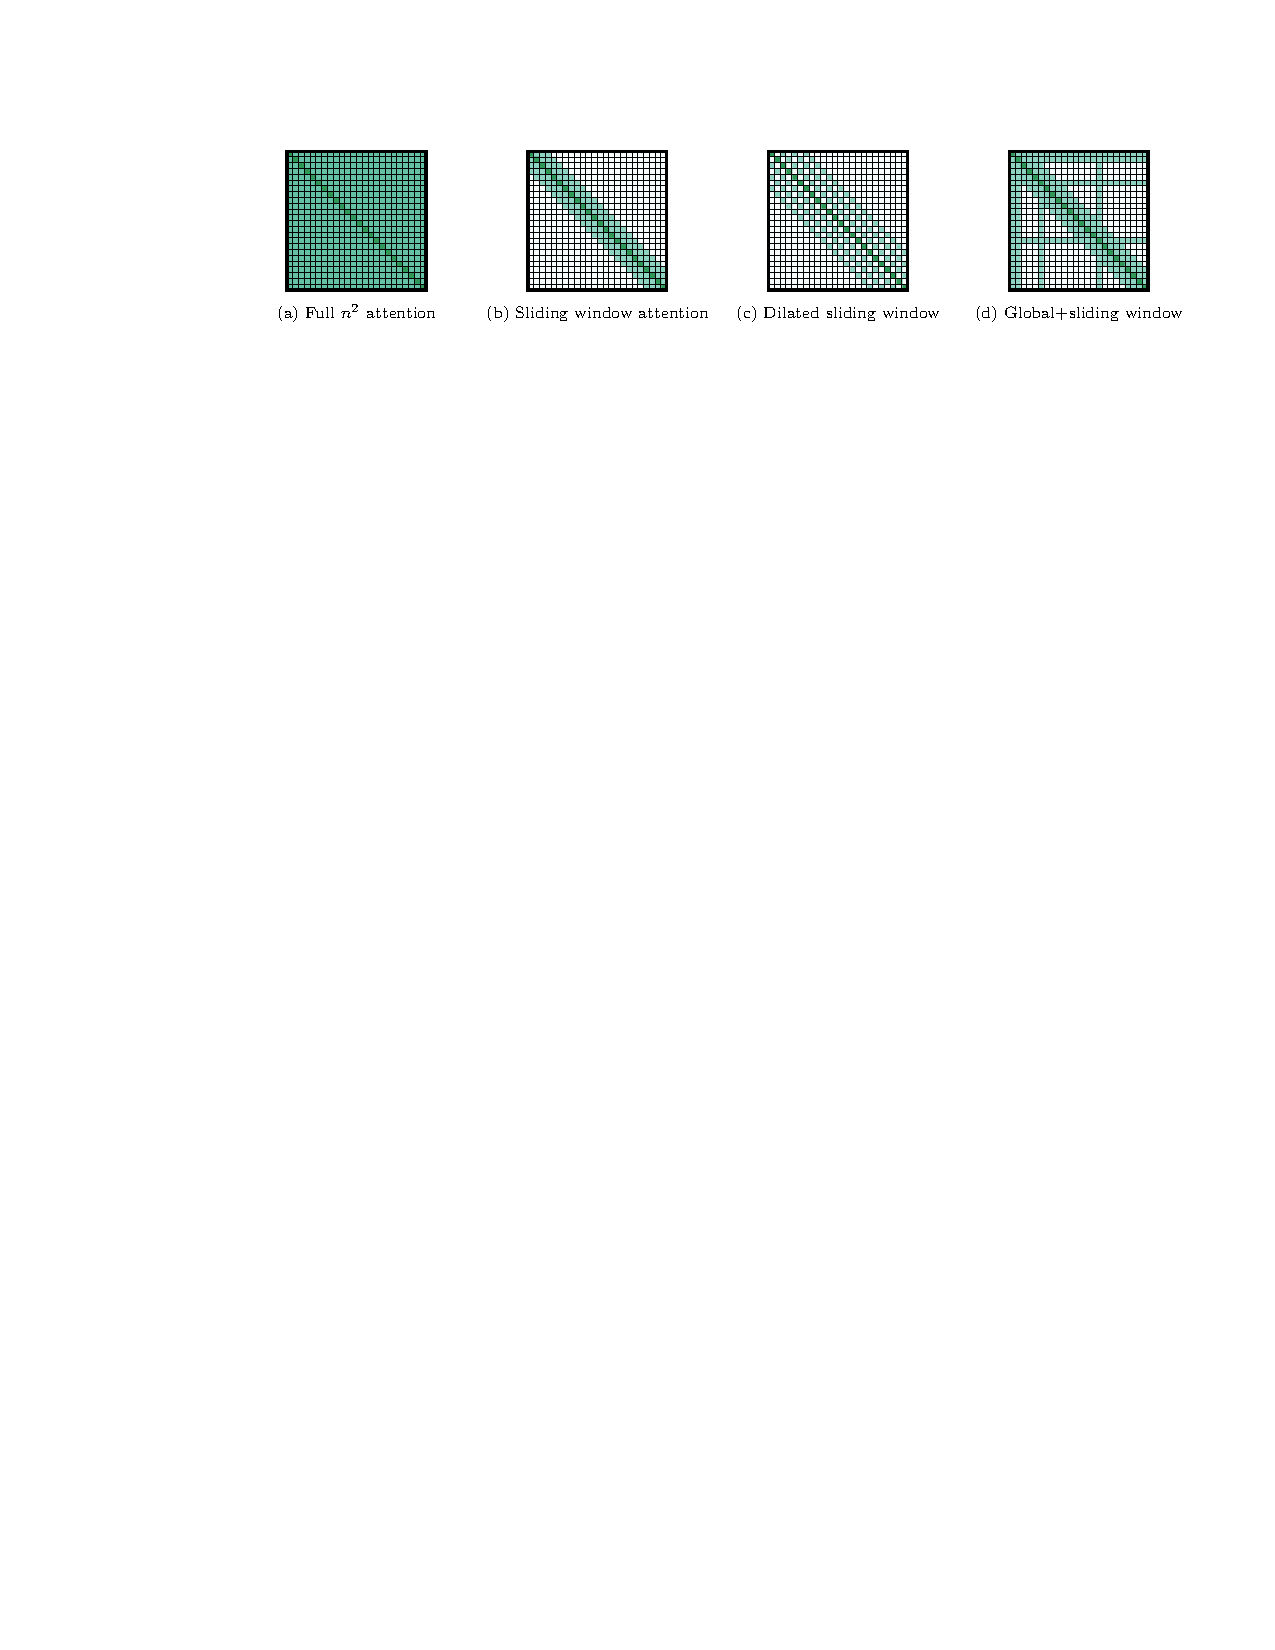
\includegraphics[width=\textwidth]{longformer_attention.pdf}
        \caption[Longformer Attention Patterns]{Original attention and Longormer attention patterns. Reprinted from \citep{longformer}.}
        \label{fig:longformer_attention}
\end{figure}

To utilize the benefits of this sparsified attention, the authors had to implement a custom CUDA kernel capable of computing parts of matrix multiplication effectively. 

\subsubsection{Reformer}

Reformer architecture \citep{reformer} offers two changes to the transformer model.
The first is the usage of locality-sensitive hashing (LSH) \citep{lsh} in the attention mechanism, and the second is the use of reversible residual networks (RevNets) \citep{revnets}.

The main idea behind the Reformer's attention is that softmax output from Equation \ref{eq:attention} is influenced most by the largest values of $QK^T$. 
Since the output of $QK^T$ represents the dot products between the rows of $Q$ and $K$, the largest values are those, for which are the vectors from $Q$ and $K$ closest to each other.
The problem of finding the closest vectors is still in $\bigO(n^2)$ since we need to compute the cosine distance between all the vector pairs -- we would need to compute $QK^T$ nonetheless. %??? TODO check grammar
Here the authors utilize LSH for finding the closest vectors.
Hash function $h(x)$ is locality-sensitive if it maps nearby vectors to the same hash with high probability. 
The simplified base idea is that under random linear projections (randomly initialized matrix) into $n_{buckets}$ dimensional space, nearby vectors preserve their orientation, thus sharing the index of the dimension where they show the highest values.
Multiple random projections are performed in parallel to reduce the probability of similar vectors differing in the maximal indices.
After the LSH computation is finished, each vector has been assigned to a ``bucket''.
Then the matrix $Q$ is sorted so that vectors from the same buckets are in a sequence.
What follows is the computation of full attention, but only on parts of the sorted matrix.
The parts are selected so that each bucket attends to all of the vectors in the bucket and one previous bucket, see Figure \ref{fig:reformer_buckets}.
The authors also noted that setting $Q=K$ did not negatively impact the model's performance, and therefore LSH is applied only to the matrix $Q$.

Another way to look at the LSH bucketing is to compute the dot product of the input vectors with a sequence of $\dfrac{n_{buckets}}{2}$ random vectors followed by their negative counterparts, of the same dimension as the input vectors.
Since cosine-similar vectors produce the highest values of dot products, we can be confident that vectors are similar if they shared the highest dot product values with the same random vectors even after multiple rounds of these projections.

\begin{figure}[!htb]
        \centering
        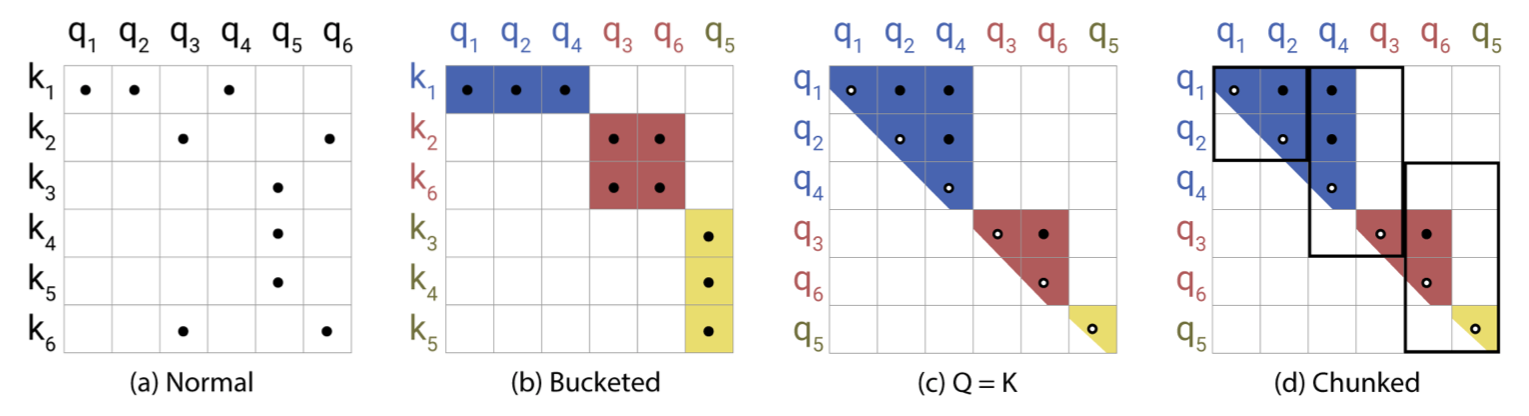
\includegraphics[width=\textwidth]{reformer_buckets.png}
        \caption[Reformer Attention Visualization]{Reformer attention buckets. Reprinted from \citep{reformer}.}
        \label{fig:reformer_buckets}
\end{figure}

In order to reduce the memory complexity, the Reformer model applies three methods.
The first one is the use of RevNets \citep{revnets} discarding the need for storing layers' activations (Figure \ref{fig:revnets}). The second one is the use of ``chunking'' -- feeding only ``chunks'' of input at a time through the linear layers.
The last one is the swapping of the parameters of the currently unused layer from GPU to CPU. This would not be efficient in normal transformers, but since Reformer is able to work with inputs even 64,000 tokens long, the authors claim that ``the amount of compute done with the parameters amortizes the cost of their transfer.''

\begin{figure}[!htb]
        \centering
        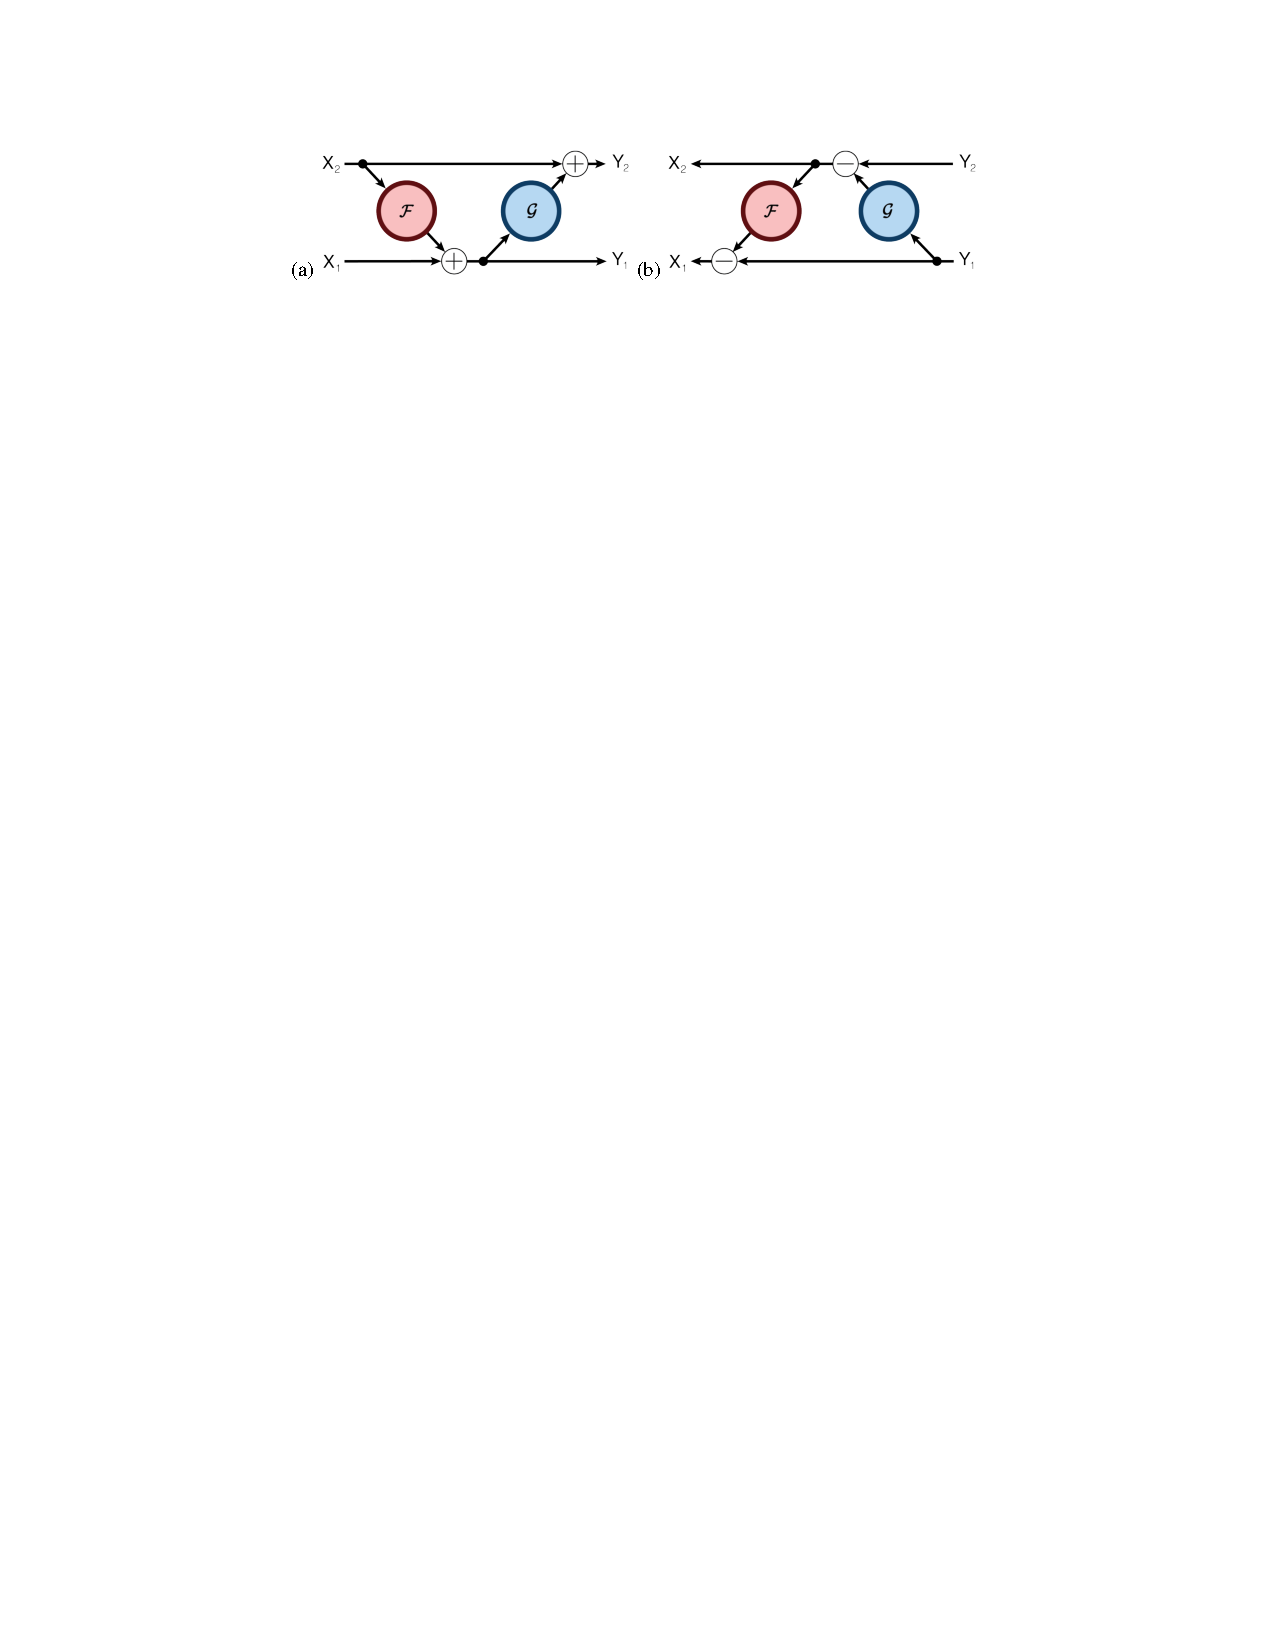
\includegraphics{revnets.pdf}
        \caption[RevNet Scheme]{The forward \textbf{(a)} and the backward \textbf{(b)} computations scheme of a residual block. Reprinted from \citep{revnets}.}
        \label{fig:revnets}
\end{figure}

\subsubsection{Performer}

Performer model \citep{performer} looks at the self-attention mechanism, concretely at the softmax substep $A=\exp(\frac{QK^T}{\sqrt{d}})$, as a randomized kernel function: 
\begin{equation}
    A_{i,j}=K(q_i,k_j)=\mathbb{E}[\phi(q_i)^T\phi(k_j)]\ ,
\end{equation}
where K is a kernel function $K\colon\R^d\times\R^d\rightarrow\R$ defined for a feature map $\phi\colon\R^d\rightarrow\R^r$.
The authors approximate the attention by using the randomized feature map to define matrices $Q', K'\in\R^{n\times r}$, with the rows equal to $\phi(q_i^T)^T$ and $\phi(k_i^T)^T$, respectively.
Then, by calculating in the paranthesized order
\begin{equation}
        AV = (Q'(K'V))
\end{equation}
the authors reduce the time complexity from $\bigO(n^2d)$ to $\bigO(nrd)$.
The paper then deals with finding suitable randomized feature maps with adequate theoretical assurances. 
The authors propose a general form
\begin{equation}
        \phi(x)=\frac{h(x)}{\sqrt{m}}(f_1(\omega_1^Tx),\dots,f_1(\omega_m^Tx),
        \dots,f_l(\omega_1^Tx),\dots,f_l(\omega_m^Tx))\ ,
\end{equation}
where $f_1,\dots,f_l\colon\R\rightarrow\R$, $g\colon\R^d\rightarrow\R$ and $\omega_1,\dots,\omega_m\overset{\text{iid}}{\sim}\mathcal{D}$ for some distribution $\mathcal{D}\in\powerset{\R}^d$.

The authors conclude their theoretical research by guaranteeing ``unbiased or nearly-unbiased estimation of the attention matrix, uniform convergence and low estimation variance'' for $h(x)=\exp(\frac{||x||}{2})$, $l=2$, $f_1=\cos$, $f_2=\sin$, $\mathcal{D}=\mathcal{N}(0,\textbf{I}_d)$, and ensuring that $\omega_1,\dots,\omega_m$ are perpendicular to each other, \citep[Theorem 4]{performer}.
The parameter $m$ does depend on the L2-norm of the queries and keys, the dimensionality of the embeddings, and the required precision, but does not depend on the input sequence length $n$.

\subsubsection{\nystr{}}

Nystr\"omformer's \citep{nystrom} base idea is to approximate the attention computation by subsampling the original $Q$ and $K$ matrices and using Nystr\"om-based method to approximate the full attention. 
The subsampling is done by splitting the $Q$ and $K$ matrices into equal parts and then averaging each part into single vectors, calling them landmarks.

The full attention matrix can be written as
\begin{equation}
        \text{Attention}(Q,K,V)=\text{softmax}\left(\frac{QK^T}{\sqrt{d}}\right)V=
        \begin{bmatrix}
                A_S && B_S \\
                F_S && C_S
        \end{bmatrix}V\ ,
\end{equation}
where $A_S\in\R^{m\times m}$ and other matrices are of appropriate shapes, with $m$ being the number of samples (landmarks). 
One could approximate the attention by expressing the matrix $C_S$ using the other matrices: $C_S=F_SA_S^+B_S$. The $+$ sign indicates the Moore-Penrose inverse.

Such usage of Nystr\"om approximation will not help, as the samples can only be obtained after the attention matrix is computed -- the softmax operation needs the whole matrix $QK^T$ (or at least its rows) to be complete. 
Nevertheless, the authors do compute softmax over only the subsampled parts of the $QK^T$ matrix and use the resulting softmax-ed matrices to compute the approximated attention.
The final approximated attention is obtained by 
\begin{equation}
        \widehat{\text{Attn}}(Q,K,V)=
        \left(
        \text{softmax}\left(\frac{Q\tilde{K}^T}{\sqrt{d}}\right)
        \text{softmax}\left(\frac{\tilde{Q}\tilde{K}^T}{\sqrt{d}}\right)^+
        \right)
        \left(
        \text{softmax}\left(\frac{\tilde{Q}K^T}{\sqrt{d}}\right)
        V
        \right)
        \ ,
\end{equation}
where $\sim$ indicates a subsampled matrix. The parenthesization ensures that the computation remains efficient. The final memory and time complexity is $\bigO(n)$, provided $m\ll n$.

The only theoretical guarantee presented directly in the paper is that if the landmarks are equal to the original keys and queries, then the approximation converges to the true attention. 
However, this holds trivially.
Proper theoretical guarantees are located in the appended repository\footnote{\url{https://github.com/mlpen/Nystromformer/}}.
There, the difference between true attention and the approximation is bounded by:
\begin{equation}
        ||\text{Attn}-\widehat{\text{Attn}}||_\infty\leq(1+||A^+_S||_\infty+||A^+_S-Z^*||_\infty)||V||_\infty\ ,
\end{equation}
where $||\cdot||_\infty$ is the maximum absolute column sum and $Z^*$ is the result of the GPU-compatible iterative algorithm \citep{iterative-moore} used by the authors to compute the Moore-Penrose inverse.
The authors report good results on various tasks, even though the softmax operation is performed on submatrices only. 
The adverse effects might be reduced by the fact that landmarks are calculated as segment means, and therefore, the original information is present during the softmax step.
Figure \ref{fig:nystrom_example} provides anecdotal comparison between full self-attention and the approximated attention.

\begin{figure}[!htb]
        \centering
        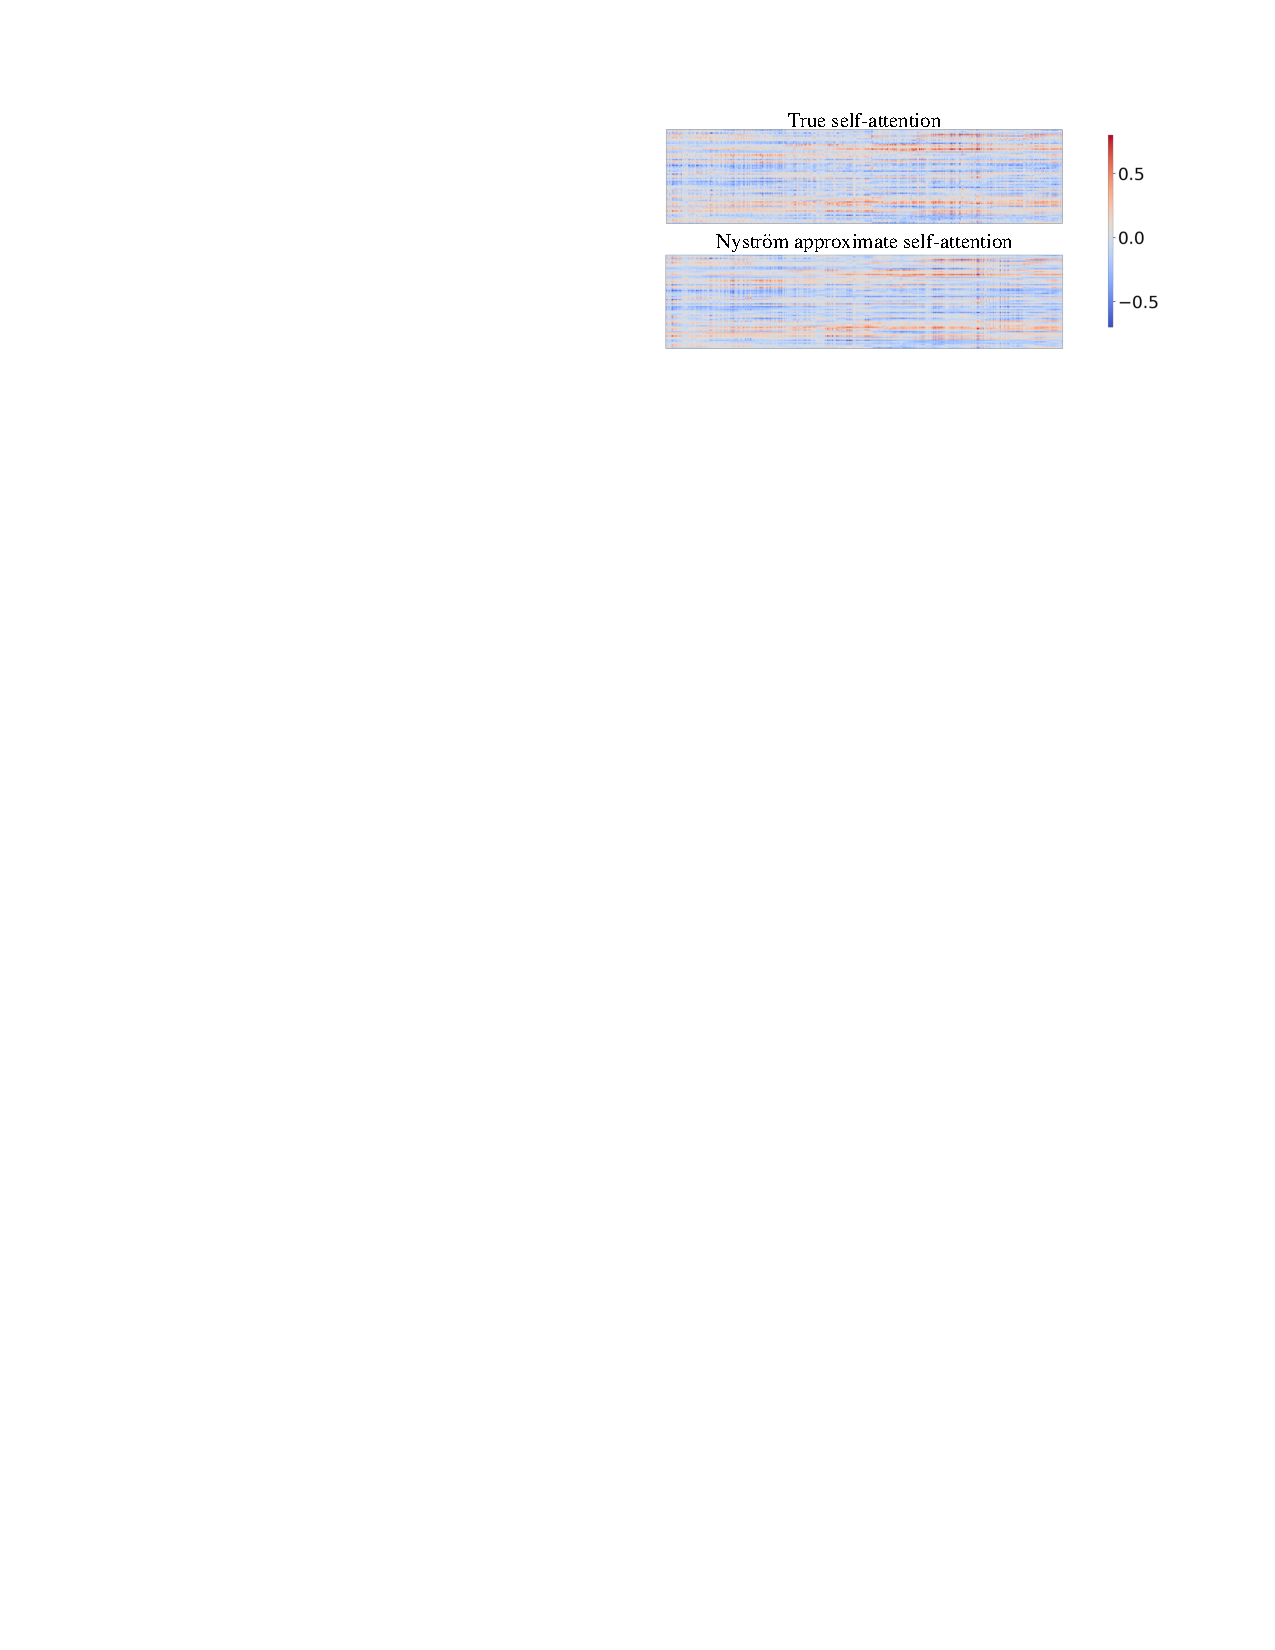
\includegraphics{nystrom_example.pdf}
        \caption[\nystr{} Attention Example]{Anecdotal comparision of the true attention and Nystr\"om approximation. Reprinted from \citep{nystrom}.}
        \label{fig:nystrom_example}
\end{figure}

The authors note that thanks to the theoretical results from \citep{nystr-2017} and \citep{linformer}, even a small number of landmarks suffices to provide a good approximation.
The first paper states that the error of Nystr\"om approximation decreases with the matrix's rank.
In the second paper, the authors suggest that the attention mechanism produces low-rank matrices.  

\subsection{Encoder Utilization in Document Retrieval}

We have, so far, introduced the encoder model, but we have yet to describe how to use it in document retrieval. We can look at the neural-model-generated encodings in a way similar to the traditional approaches.

Traditional approaches result in a sparse representation of the knowledge base with the feature dimensionality equal to the corpus's vocabulary size (the vocabulary can also contain n-grams or character n-grams if it is advantageous).
Therefore, it can be considered a weighting scheme, assigning "importance" to each word present in the document. 
% Neural approaches in this paper produce a dense representation -- a fixed-size vector of real numbers, inherently hard to interpret.

Neural approaches in this paper generate a fixed-length real-valued vector representation for both the query and all the documents in the knowledge base.
The dense representation is inherently hard to interpret, and the meaning can be derived only from the relative position of different documents' representations (vectors).
Hence the $f(q,d)$ score from Equation \ref{eq:formal_descr_dr} is the distance between the vector representations of $q$ and $d$.
The distance metric used may be cosine similarity, dot product, or some fast approximation such as FAISS \citep{faiss}.
This approach allows us to preprocess the whole knowledge base, allowing us to compute only the query representation during runtime.
The disadvantage is that we do not utilize the attention mechanism to consider each query-document relation individually and, today less relevant problem, the need for additional space to store the precomputed representation.

Neural models can also be used directly as the scoring function as in Equation \ref{eq:formal_descr_dr} and use the document-query pair $(d,q)$ as their input (the cross-attention model).
This can, according to \citet{two-tower}, lead to better performance. However, since the query is provided at runtime, the evaluation cannot be precomputed and has to run for every document each time we enter a new query.
Because of that, and because of the large number of documents in the knowledge base, this approach is unfit for real-world application.

There exists a hybrid approach capable of utilizing the cross-attention model. 
It runs the model on a small subset of the corpus, typically pre-selected by a non-neural model.
The model only reranks the gathered sentences.
Our colleague \citet{dedkova} provides a detailed look into the use of such methods in Czech document retrieval.

% i did not mention it
%As mentioned above, when dealing with natural language processing, we can approach the task in two different ways, both described in detail by \cite{two-tower}. 

%USED ABOVE
%The first is to have the document-query pair $(d,q)$ on the input of the neural model (cross-attention model).
%One of the benefits is the direct usage of the neural model on the downstream tasks, possibly granting better performance.

%USED ABOVE
%The second approach generates a fixed-length real-valued vector representation for both the query and all the documents in the knowledge base.
%Then the $f(q,d)$ score is the distance between $q$'s and $d$'s representation.
%The distance metric used may be cosine similarity, dot product, or some approximation such as FAISS \citep{faiss}.

%BLAH SOUNDS TOO SIMPLE The second approach is to preprocess the whole database of documents by the model and then using some metric for choosing the documents related to the query based on the computed representation.
%The obvious advantage is the offline preprocessing and thus improved performance during inference.
%Only the unseen query has to be processed by the neural model followed by computing the metric between the documents' representation and the query representation.
%This approach grants significant speedup compared to computing the score for every query-document pair. 

%USED ABOVE
%We will be using the second approach since the number of documents in our knowledge base renders the cross-attention paradigm computationally unfit for real-world application.
% TODO vymazat, 
%In order to solve the document retrieval task, we will focus on finding an appropriate function $f$.
%In this thesis, that means a function suitable for long documents.

\subsubsection{Generating Representations}

Generating the dense representations, also called embeddings since we project the input into a vector space with a specific dimension, is, in general, a well-studied area of research. We restrict ourselves to neural methods described in Section \ref{sec:neural_approaches}. 

There are multiple ways to generate the input's embedding from the model-processed tokens.
Sentence-BERT \citep{sbert} adds a pooling layer, either \texttt{MAX} or \texttt{MEAN}, and fine-tunes the model using two different approaches, depending on the task.
For regression tasks, TODO.
They compare their method against averaging all the output tokens' representations, selecting the out representation of special input token \texttt{[CLS]} situated at the front of the input, and against averaging input tokens' GloVe \citep{glove} word vectors.
The authors note that if the fine-tuning step is not performed, the BERT model provides little to no improvement to averaging input tokens' word vectors.

The authors of \citep{two-tower} proposed a different approach, designed directly for the task of document retrieval, in their case, over Wikipedia articles. 
They apply a fully-connected linear layer to the \texttt{[CLS]} token's representation and also pre-train the BERT model on three additional document retrieval tasks:
\begin{itemize}
        \item \textbf{Inverse Cloze Task (ICT)} - Training the model to embed sentences close to the paragraph from which they were selected. The selected sentences are omitted from the paragraph in the training step.
        \item \textbf{Body First Selection (BFS)} - Training the model to embed sentences close to the paragraphs in the same article. The sentences are selected in such a manner to reasonably expect this task to succeed. In the case of training on Wikipedia, the sentences are selected from the first paragraph (summary).
        \item \textbf{Wiki Link Prediction (WLP)} - Training the model to embed sentences close to Wikipedia articles from which there exists a hyperlink to the article of the sentence.
\end{itemize}
The authors reported significant improvements compared to using only MLM for the pre-training phase.
% USED ABOVE They use the model's final representation of the special input token \verb{[CLS]}, situated at the front of the input, as the representation of the whole input. 

\subsection{Czech Language}

TODO
%The introduced BERT-based models are seldom trained on Czech data.

\subsection{Distillation}

TODO